\documentclass[twoside]{book}

% Packages required by doxygen
\usepackage{calc}
\usepackage{doxygen}
\usepackage{graphicx}
\usepackage[utf8]{inputenc}
\usepackage{makeidx}
\usepackage{multicol}
\usepackage{multirow}
\usepackage{textcomp}
\usepackage[table]{xcolor}

% Font selection
\usepackage[T1]{fontenc}
\usepackage{mathptmx}
\usepackage[scaled=.90]{helvet}
\usepackage{courier}
\usepackage{amssymb}
\usepackage{sectsty}
\renewcommand{\familydefault}{\sfdefault}
\allsectionsfont{%
  \fontseries{bc}\selectfont%
  \color{darkgray}%
}
\renewcommand{\DoxyLabelFont}{%
  \fontseries{bc}\selectfont%
  \color{darkgray}%
}

% Page & text layout
\usepackage{geometry}
\geometry{%
  a4paper,%
  top=2.5cm,%
  bottom=2.5cm,%
  left=2.5cm,%
  right=2.5cm%
}
\tolerance=750
\hfuzz=15pt
\hbadness=750
\setlength{\emergencystretch}{15pt}
\setlength{\parindent}{0cm}
\setlength{\parskip}{0.2cm}
\makeatletter
\renewcommand{\paragraph}{%
  \@startsection{paragraph}{4}{0ex}{-1.0ex}{1.0ex}{%
    \normalfont\normalsize\bfseries\SS@parafont%
  }%
}
\renewcommand{\subparagraph}{%
  \@startsection{subparagraph}{5}{0ex}{-1.0ex}{1.0ex}{%
    \normalfont\normalsize\bfseries\SS@subparafont%
  }%
}
\makeatother

% Headers & footers
\usepackage{fancyhdr}
\pagestyle{fancyplain}
\fancyhead[LE]{\fancyplain{}{\bfseries\thepage}}
\fancyhead[CE]{\fancyplain{}{}}
\fancyhead[RE]{\fancyplain{}{\bfseries\leftmark}}
\fancyhead[LO]{\fancyplain{}{\bfseries\rightmark}}
\fancyhead[CO]{\fancyplain{}{}}
\fancyhead[RO]{\fancyplain{}{\bfseries\thepage}}
\fancyfoot[LE]{\fancyplain{}{}}
\fancyfoot[CE]{\fancyplain{}{}}
\fancyfoot[RE]{\fancyplain{}{\bfseries\scriptsize Generated on Thu Mar 31 2016 18\-:54\-:44 for My Project by Doxygen }}
\fancyfoot[LO]{\fancyplain{}{\bfseries\scriptsize Generated on Thu Mar 31 2016 18\-:54\-:44 for My Project by Doxygen }}
\fancyfoot[CO]{\fancyplain{}{}}
\fancyfoot[RO]{\fancyplain{}{}}
\renewcommand{\footrulewidth}{0.4pt}
\renewcommand{\chaptermark}[1]{%
  \markboth{#1}{}%
}
\renewcommand{\sectionmark}[1]{%
  \markright{\thesection\ #1}%
}

% Indices & bibliography
\usepackage{natbib}
\usepackage[titles]{tocloft}
\setcounter{tocdepth}{3}
\setcounter{secnumdepth}{5}
\makeindex

% Hyperlinks (required, but should be loaded last)
\usepackage{ifpdf}
\ifpdf
  \usepackage[pdftex,pagebackref=true]{hyperref}
\else
  \usepackage[ps2pdf,pagebackref=true]{hyperref}
\fi
\hypersetup{%
  colorlinks=true,%
  linkcolor=blue,%
  citecolor=blue,%
  unicode%
}

% Custom commands
\newcommand{\clearemptydoublepage}{%
  \newpage{\pagestyle{empty}\cleardoublepage}%
}


%===== C O N T E N T S =====

\begin{document}

% Titlepage & ToC
\hypersetup{pageanchor=false}
\pagenumbering{roman}
\begin{titlepage}
\vspace*{7cm}
\begin{center}%
{\Large My Project }\\
\vspace*{1cm}
{\large Generated by Doxygen 1.8.6}\\
\vspace*{0.5cm}
{\small Thu Mar 31 2016 18:54:44}\\
\end{center}
\end{titlepage}
\clearemptydoublepage
\tableofcontents
\clearemptydoublepage
\pagenumbering{arabic}
\hypersetup{pageanchor=true}

%--- Begin generated contents ---
\chapter{Namespace Index}
\section{Namespace List}
Here is a list of all documented namespaces with brief descriptions\-:\begin{DoxyCompactList}
\item\contentsline{section}{\hyperlink{namespaceed}{ed} }{\pageref{namespaceed}}{}
\end{DoxyCompactList}

\chapter{Hierarchical Index}
\section{Class Hierarchy}
This inheritance list is sorted roughly, but not completely, alphabetically\-:\begin{DoxyCompactList}
\item \contentsline{section}{ed\-:\-:Donante\-Interfaz}{\pageref{classed_1_1DonanteInterfaz}}{}
\begin{DoxyCompactList}
\item \contentsline{section}{ed\-:\-:Donante}{\pageref{classed_1_1Donante}}{}
\end{DoxyCompactList}
\end{DoxyCompactList}

\chapter{Class Index}
\section{Class List}
Here are the classes, structs, unions and interfaces with brief descriptions\-:\begin{DoxyCompactList}
\item\contentsline{section}{\hyperlink{classed_1_1Donante}{ed\-::\-Donante} \\*Defición de la clase \hyperlink{classed_1_1Donante}{Donante} }{\pageref{classed_1_1Donante}}{}
\item\contentsline{section}{\hyperlink{classed_1_1DonanteInterfaz}{ed\-::\-Donante\-Interfaz} \\*Definición de la clase \hyperlink{classed_1_1DonanteInterfaz}{Donante\-Interfaz} }{\pageref{classed_1_1DonanteInterfaz}}{}
\end{DoxyCompactList}

\chapter{File Index}
\section{File List}
Here is a list of all documented files with brief descriptions\-:\begin{DoxyCompactList}
\item\contentsline{section}{{\bfseries donante.\-hpp} }{\pageref{donante_8hpp}}{}
\item\contentsline{section}{{\bfseries donante\-Interfaz.\-hpp} }{\pageref{donanteInterfaz_8hpp}}{}
\item\contentsline{section}{\hyperlink{funciones_8cpp}{funciones.\-cpp} \\*Código de las funciones utilizadas en el menú }{\pageref{funciones_8cpp}}{}
\item\contentsline{section}{\hyperlink{funciones_8hpp}{funciones.\-hpp} \\*Prototipos de las funciones utilizadas en el menú }{\pageref{funciones_8hpp}}{}
\item\contentsline{section}{\hyperlink{macros_8hpp}{macros.\-hpp} \\*Macros para el diseño de pantallas }{\pageref{macros_8hpp}}{}
\end{DoxyCompactList}

\chapter{Namespace Documentation}
\hypertarget{namespaceed}{\section{ed Namespace Reference}
\label{namespaceed}\index{ed@{ed}}
}
\subsection*{Classes}
\begin{DoxyCompactItemize}
\item 
class \hyperlink{classed_1_1Donante}{Donante}
\begin{DoxyCompactList}\small\item\em Defición de la clase \hyperlink{classed_1_1Donante}{Donante}. \end{DoxyCompactList}\item 
class \hyperlink{classed_1_1DonanteInterfaz}{Donante\-Interfaz}
\begin{DoxyCompactList}\small\item\em Definición de la clase \hyperlink{classed_1_1DonanteInterfaz}{Donante\-Interfaz}. \end{DoxyCompactList}\end{DoxyCompactItemize}
\subsection*{Functions}
\begin{DoxyCompactItemize}
\item 
ostream \& \hyperlink{namespaceed_a2f863e2611a159ce8c43a30836febb8c}{operator$<$$<$} (ostream \&stream, \hyperlink{classed_1_1Donante}{Donante} const \&p)
\item 
istream \& \hyperlink{namespaceed_aded1507a91c2b68863018cdc56aec49e}{operator$>$$>$} (istream \&stream, \hyperlink{classed_1_1Donante}{Donante} \&p)
\end{DoxyCompactItemize}


\subsection{Detailed Description}
\begin{DoxyAttention}{Attention}
Se incluye la clase \hyperlink{classed_1_1Donante}{Donante} dentro del espacio de nombres ed 
\end{DoxyAttention}


\subsection{Function Documentation}
\hypertarget{namespaceed_a2f863e2611a159ce8c43a30836febb8c}{\index{ed@{ed}!operator$<$$<$@{operator$<$$<$}}
\index{operator$<$$<$@{operator$<$$<$}!ed@{ed}}
\subsubsection[{operator$<$$<$}]{\setlength{\rightskip}{0pt plus 5cm}ostream\& ed\-::operator$<$$<$ (
\begin{DoxyParamCaption}
\item[{ostream \&}]{stream, }
\item[{{\bf Donante} const \&}]{p}
\end{DoxyParamCaption}
)}}\label{namespaceed_a2f863e2611a159ce8c43a30836febb8c}
\begin{DoxyAttention}{Attention}
Funcion amiga de la clase \hyperlink{classed_1_1Donante}{Donante} 
\end{DoxyAttention}

\begin{DoxyParams}{Parameters}
{\em stream} & ostream, flujo de salida \\
\hline
{\em p} & \hyperlink{classed_1_1Donante}{Donante}, pasado por referencia constante \\
\hline
\end{DoxyParams}
\begin{DoxyPrecond}{Precondition}
El donante debe existir 
\end{DoxyPrecond}
\begin{DoxyPostcond}{Postcondition}
Se escribe por pantalla los datos del donante 
\end{DoxyPostcond}
\begin{DoxySeeAlso}{See Also}
operator $>$$>$ 
\end{DoxySeeAlso}
\hypertarget{namespaceed_aded1507a91c2b68863018cdc56aec49e}{\index{ed@{ed}!operator$>$$>$@{operator$>$$>$}}
\index{operator$>$$>$@{operator$>$$>$}!ed@{ed}}
\subsubsection[{operator$>$$>$}]{\setlength{\rightskip}{0pt plus 5cm}istream\& ed\-::operator$>$$>$ (
\begin{DoxyParamCaption}
\item[{istream \&}]{stream, }
\item[{{\bf Donante} \&}]{p}
\end{DoxyParamCaption}
)}}\label{namespaceed_aded1507a91c2b68863018cdc56aec49e}
\begin{DoxyAttention}{Attention}
Funcion amiga de la clase \hyperlink{classed_1_1Donante}{Donante} 
\end{DoxyAttention}

\begin{DoxyParams}{Parameters}
{\em stream} & istream, flujo de entrada \\
\hline
{\em p} & \hyperlink{classed_1_1Donante}{Donante}, pasado por referencia \\
\hline
\end{DoxyParams}
\begin{DoxyPrecond}{Precondition}
El monomio debe existir 
\end{DoxyPrecond}
\begin{DoxyPostcond}{Postcondition}
Se lee por teclado los datos de un donante 
\end{DoxyPostcond}
\begin{DoxySeeAlso}{See Also}
operator $<$$<$ 
\end{DoxySeeAlso}

\chapter{Class Documentation}
\hypertarget{classed_1_1Donante}{\section{ed\-:\-:Donante Class Reference}
\label{classed_1_1Donante}\index{ed\-::\-Donante@{ed\-::\-Donante}}
}


Defición de la clase \hyperlink{classed_1_1Donante}{Donante}.  




{\ttfamily \#include $<$donante.\-hpp$>$}

Inheritance diagram for ed\-:\-:Donante\-:\begin{figure}[H]
\begin{center}
\leavevmode
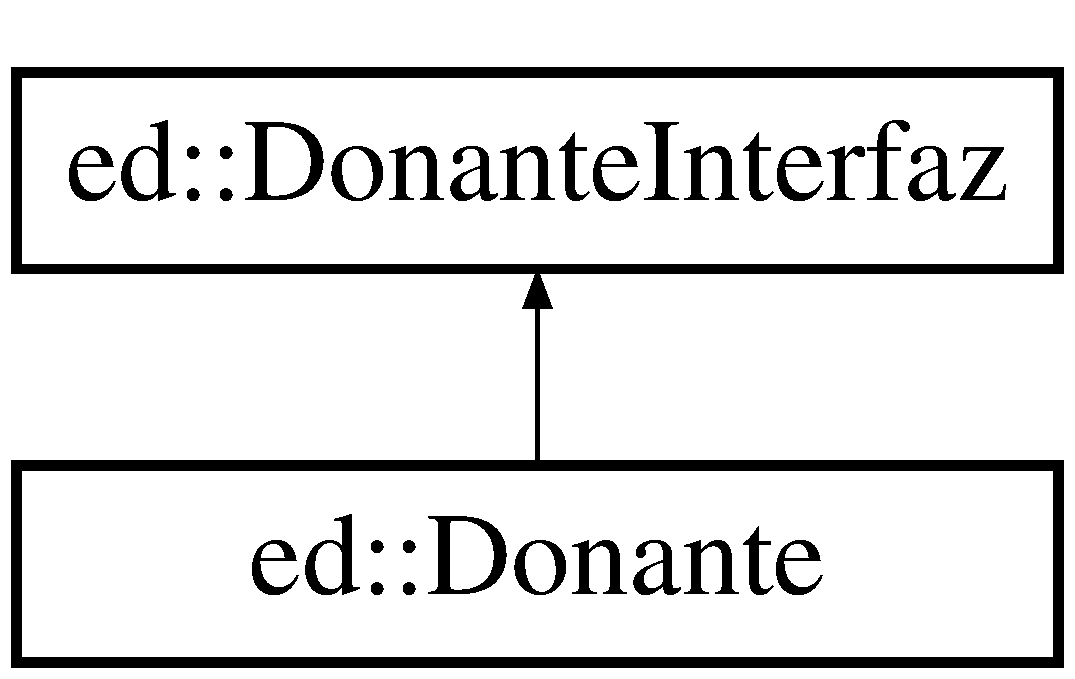
\includegraphics[height=2.000000cm]{classed_1_1Donante}
\end{center}
\end{figure}
\subsection*{Constructores de la clase Donante}
\begin{DoxyCompactItemize}
\item 
\hyperlink{classed_1_1Donante_ab60c71e2630bce8681331aadf024bced}{Donante} (string nombre=\char`\"{}\char`\"{}, string apellido=\char`\"{}\char`\"{}, string grupo\-Sanguineo=\char`\"{}\char`\"{}, string factor\-R\-H=\char`\"{}\char`\"{})
\begin{DoxyCompactList}\small\item\em Contructor que crea un donante por defecto. \end{DoxyCompactList}\item 
\hyperlink{classed_1_1Donante_a10e4c4449297d461df58b6adb3765584}{Donante} (\hyperlink{classed_1_1Donante}{Donante} const \&p)
\begin{DoxyCompactList}\small\item\em Contructor que crea un donante a partir de otro donante. \end{DoxyCompactList}\item 
void \hyperlink{classed_1_1Donante_a346b31e40b478d25c3e311de2ff2fb2c}{set\-Nombre} (const string \&nombre)
\begin{DoxyCompactList}\small\item\em Asigna un valor \char`\"{}nombre\char`\"{} al nombre de un donante. \end{DoxyCompactList}\item 
void \hyperlink{classed_1_1Donante_ae1404d01bdc865c03bfc179b408df4d7}{set\-Apellido} (const string \&apellido)
\begin{DoxyCompactList}\small\item\em Asigna un valor \char`\"{}apellido\char`\"{} al apellido de un donante. \end{DoxyCompactList}\item 
void \hyperlink{classed_1_1Donante_a24dcea06d8dd84d596e115b8c94e8eb2}{set\-Grupo\-Sanguineo} (const string \&grupo\-Sanguineo)
\begin{DoxyCompactList}\small\item\em Asigna un valor \char`\"{}grupo\-Sanguineo\char`\"{} al grupo\-Sanguineo de un donante. \end{DoxyCompactList}\item 
void \hyperlink{classed_1_1Donante_a724f1dcdf7a3cf78fd80151b30038c74}{set\-Factor\-R\-H} (const string \&factor\-R\-H)
\begin{DoxyCompactList}\small\item\em Asigna un valor \char`\"{}factor\-R\-H\char`\"{} al factor\-R\-H de un donante. \end{DoxyCompactList}\item 
string \hyperlink{classed_1_1Donante_a6ee5ef3051ee5e87aecefbbb68907d4a}{get\-Nombre} () const 
\begin{DoxyCompactList}\small\item\em Devuelve el nombre de un donante. \end{DoxyCompactList}\item 
string \hyperlink{classed_1_1Donante_a3c47b3238b610ea3541161bc1a90d9f8}{get\-Apellido} () const 
\begin{DoxyCompactList}\small\item\em Devuelve el apellido de un donante. \end{DoxyCompactList}\item 
string \hyperlink{classed_1_1Donante_a6a6d49990afd2da9908df86462457049}{get\-Grupo\-Sanguineo} () const 
\begin{DoxyCompactList}\small\item\em Devuelve el grupo sanguineo de un donante. \end{DoxyCompactList}\item 
string \hyperlink{classed_1_1Donante_a61c107f22340497f4bf5169997be5ddc}{get\-Factor\-R\-H} () const 
\begin{DoxyCompactList}\small\item\em Devuelve el factor R\-H de un donante. \end{DoxyCompactList}\item 
\hyperlink{classed_1_1Donante}{Donante} \& \hyperlink{classed_1_1Donante_af8cc31baf86b839a5b08b15d52da31a4}{operator=} (\hyperlink{classed_1_1Donante}{Donante} const \&p)
\begin{DoxyCompactList}\small\item\em Operador de copia de un donante en otro. \end{DoxyCompactList}\item 
bool \hyperlink{classed_1_1Donante_ad573bdc55211e23bcb2c6906a5d64f6b}{operator==} (\hyperlink{classed_1_1Donante}{Donante} const \&p)
\begin{DoxyCompactList}\small\item\em Operador de comparacion de igualdad. \end{DoxyCompactList}\item 
bool \hyperlink{classed_1_1Donante_aedaee5673a9c9f5fef2e94d3d3383b27}{operator$<$=} (\hyperlink{classed_1_1Donante}{Donante} const \&p)
\begin{DoxyCompactList}\small\item\em Operador de comparacion. \end{DoxyCompactList}\item 
void \hyperlink{classed_1_1Donante_a6eaca430e33a875ea87b65d7b755d24d}{escribir\-Donante} ()
\begin{DoxyCompactList}\small\item\em Escribe los datos de un donante por pantalla. \end{DoxyCompactList}\item 
void \hyperlink{classed_1_1Donante_abbf8fc955836761e5efec2c888a87032}{leer\-Donante} ()
\begin{DoxyCompactList}\small\item\em Asigna lee por teclado los datos de un donante. \end{DoxyCompactList}\item 
ostream \& \hyperlink{classed_1_1Donante_abf722a02c1261a0148fd3529ecbb0d0a}{operator$<$$<$} (ostream \&stream, \hyperlink{classed_1_1Donante}{Donante} const \&p)
\begin{DoxyCompactList}\small\item\em Sobrecarga del operador de salida \char`\"{}$<$$<$\char`\"{}. \end{DoxyCompactList}\item 
istream \& \hyperlink{classed_1_1Donante_afab845cf76f83a496fb1862f7ca15c5f}{operator$>$$>$} (istream \&stream, \hyperlink{classed_1_1Donante}{Donante} \&p)
\begin{DoxyCompactList}\small\item\em Sobrecarga del operador de entrada \char`\"{}$>$$>$\char`\"{}. \end{DoxyCompactList}\end{DoxyCompactItemize}
\subsection*{Additional Inherited Members}


\subsection{Detailed Description}
Defición de la clase \hyperlink{classed_1_1Donante}{Donante}. 

\subsection{Constructor \& Destructor Documentation}
\hypertarget{classed_1_1Donante_ab60c71e2630bce8681331aadf024bced}{\index{ed\-::\-Donante@{ed\-::\-Donante}!Donante@{Donante}}
\index{Donante@{Donante}!ed::Donante@{ed\-::\-Donante}}
\subsubsection[{Donante}]{\setlength{\rightskip}{0pt plus 5cm}ed\-::\-Donante\-::\-Donante (
\begin{DoxyParamCaption}
\item[{string}]{nombre = {\ttfamily \char`\"{}\char`\"{}}, }
\item[{string}]{apellido = {\ttfamily \char`\"{}\char`\"{}}, }
\item[{string}]{grupo\-Sanguineo = {\ttfamily \char`\"{}\char`\"{}}, }
\item[{string}]{factor\-R\-H = {\ttfamily \char`\"{}\char`\"{}}}
\end{DoxyParamCaption}
)\hspace{0.3cm}{\ttfamily [inline]}}}\label{classed_1_1Donante_ab60c71e2630bce8681331aadf024bced}


Contructor que crea un donante por defecto. 

\begin{DoxyAttention}{Attention}
Función sobrecargada 
\end{DoxyAttention}
\begin{DoxyNote}{Note}
Los parámetros tienen valores por defecto 
\end{DoxyNote}

\begin{DoxyParams}{Parameters}
{\em nombre} & string, nombre del donante \\
\hline
{\em apellido} & string, apellido del donate \\
\hline
{\em grupo\-Sanguineo} & string, grupo sanguineo del donante \\
\hline
{\em factor\-R\-H} & string, factor R\-H del donante \\
\hline
\end{DoxyParams}
\begin{DoxyPrecond}{Precondition}
Ninguna 
\end{DoxyPrecond}
\begin{DoxyPostcond}{Postcondition}
Ninguna 
\end{DoxyPostcond}
\hypertarget{classed_1_1Donante_a10e4c4449297d461df58b6adb3765584}{\index{ed\-::\-Donante@{ed\-::\-Donante}!Donante@{Donante}}
\index{Donante@{Donante}!ed::Donante@{ed\-::\-Donante}}
\subsubsection[{Donante}]{\setlength{\rightskip}{0pt plus 5cm}ed\-::\-Donante\-::\-Donante (
\begin{DoxyParamCaption}
\item[{{\bf Donante} const \&}]{p}
\end{DoxyParamCaption}
)\hspace{0.3cm}{\ttfamily [inline]}}}\label{classed_1_1Donante_a10e4c4449297d461df58b6adb3765584}


Contructor que crea un donante a partir de otro donante. 

\begin{DoxyAttention}{Attention}
Función sobrecargada 
\end{DoxyAttention}

\begin{DoxyParams}{Parameters}
{\em p} & \hyperlink{classed_1_1Donante}{Donante}, \hyperlink{classed_1_1Donante}{Donante} pasado por referencia \\
\hline
\end{DoxyParams}
\begin{DoxyPrecond}{Precondition}
Ninguna 
\end{DoxyPrecond}
\begin{DoxyPostcond}{Postcondition}
Ninguna 
\end{DoxyPostcond}


\subsection{Member Function Documentation}
\hypertarget{classed_1_1Donante_a6eaca430e33a875ea87b65d7b755d24d}{\index{ed\-::\-Donante@{ed\-::\-Donante}!escribir\-Donante@{escribir\-Donante}}
\index{escribir\-Donante@{escribir\-Donante}!ed::Donante@{ed\-::\-Donante}}
\subsubsection[{escribir\-Donante}]{\setlength{\rightskip}{0pt plus 5cm}void Donante\-::escribir\-Donante (
\begin{DoxyParamCaption}
{}
\end{DoxyParamCaption}
)}}\label{classed_1_1Donante_a6eaca430e33a875ea87b65d7b755d24d}


Escribe los datos de un donante por pantalla. 

\begin{DoxyPrecond}{Precondition}
El donante debe existir 
\end{DoxyPrecond}
\begin{DoxyPostcond}{Postcondition}
Ninguna 
\end{DoxyPostcond}
\hypertarget{classed_1_1Donante_a3c47b3238b610ea3541161bc1a90d9f8}{\index{ed\-::\-Donante@{ed\-::\-Donante}!get\-Apellido@{get\-Apellido}}
\index{get\-Apellido@{get\-Apellido}!ed::Donante@{ed\-::\-Donante}}
\subsubsection[{get\-Apellido}]{\setlength{\rightskip}{0pt plus 5cm}string ed\-::\-Donante\-::get\-Apellido (
\begin{DoxyParamCaption}
{}
\end{DoxyParamCaption}
) const\hspace{0.3cm}{\ttfamily [inline]}, {\ttfamily [virtual]}}}\label{classed_1_1Donante_a3c47b3238b610ea3541161bc1a90d9f8}


Devuelve el apellido de un donante. 

\begin{DoxyReturn}{Returns}
Apellido de un donate 
\end{DoxyReturn}
\begin{DoxyPrecond}{Precondition}
El donante debe existir anteriormente 
\end{DoxyPrecond}
\begin{DoxyPostcond}{Postcondition}
Ninguna 
\end{DoxyPostcond}


Implements \hyperlink{classed_1_1DonanteInterfaz_af318d1ba60b3ef9450218a30e980d3a6}{ed\-::\-Donante\-Interfaz}.

\hypertarget{classed_1_1Donante_a61c107f22340497f4bf5169997be5ddc}{\index{ed\-::\-Donante@{ed\-::\-Donante}!get\-Factor\-R\-H@{get\-Factor\-R\-H}}
\index{get\-Factor\-R\-H@{get\-Factor\-R\-H}!ed::Donante@{ed\-::\-Donante}}
\subsubsection[{get\-Factor\-R\-H}]{\setlength{\rightskip}{0pt plus 5cm}string ed\-::\-Donante\-::get\-Factor\-R\-H (
\begin{DoxyParamCaption}
{}
\end{DoxyParamCaption}
) const\hspace{0.3cm}{\ttfamily [inline]}, {\ttfamily [virtual]}}}\label{classed_1_1Donante_a61c107f22340497f4bf5169997be5ddc}


Devuelve el factor R\-H de un donante. 

\begin{DoxyReturn}{Returns}
factor\-R\-H de un donante 
\end{DoxyReturn}
\begin{DoxyPrecond}{Precondition}
El donante debe existir anteriormente 
\end{DoxyPrecond}
\begin{DoxyPostcond}{Postcondition}
Ninguna 
\end{DoxyPostcond}


Implements \hyperlink{classed_1_1DonanteInterfaz_ad6137e761b69b8fd085088a7a01cf5e2}{ed\-::\-Donante\-Interfaz}.

\hypertarget{classed_1_1Donante_a6a6d49990afd2da9908df86462457049}{\index{ed\-::\-Donante@{ed\-::\-Donante}!get\-Grupo\-Sanguineo@{get\-Grupo\-Sanguineo}}
\index{get\-Grupo\-Sanguineo@{get\-Grupo\-Sanguineo}!ed::Donante@{ed\-::\-Donante}}
\subsubsection[{get\-Grupo\-Sanguineo}]{\setlength{\rightskip}{0pt plus 5cm}string ed\-::\-Donante\-::get\-Grupo\-Sanguineo (
\begin{DoxyParamCaption}
{}
\end{DoxyParamCaption}
) const\hspace{0.3cm}{\ttfamily [inline]}, {\ttfamily [virtual]}}}\label{classed_1_1Donante_a6a6d49990afd2da9908df86462457049}


Devuelve el grupo sanguineo de un donante. 

\begin{DoxyReturn}{Returns}
grupo\-Sanguineo de un polinomio 
\end{DoxyReturn}
\begin{DoxyPrecond}{Precondition}
El donante debe existir anteriormente 
\end{DoxyPrecond}
\begin{DoxyPostcond}{Postcondition}
Ninguna 
\end{DoxyPostcond}


Implements \hyperlink{classed_1_1DonanteInterfaz_a06fe986962a85b487c8e1c5525beec15}{ed\-::\-Donante\-Interfaz}.

\hypertarget{classed_1_1Donante_a6ee5ef3051ee5e87aecefbbb68907d4a}{\index{ed\-::\-Donante@{ed\-::\-Donante}!get\-Nombre@{get\-Nombre}}
\index{get\-Nombre@{get\-Nombre}!ed::Donante@{ed\-::\-Donante}}
\subsubsection[{get\-Nombre}]{\setlength{\rightskip}{0pt plus 5cm}string ed\-::\-Donante\-::get\-Nombre (
\begin{DoxyParamCaption}
{}
\end{DoxyParamCaption}
) const\hspace{0.3cm}{\ttfamily [inline]}, {\ttfamily [virtual]}}}\label{classed_1_1Donante_a6ee5ef3051ee5e87aecefbbb68907d4a}


Devuelve el nombre de un donante. 

\begin{DoxyReturn}{Returns}
Nombre de un donante 
\end{DoxyReturn}
\begin{DoxyPrecond}{Precondition}
El donante debe existir anteriormente 
\end{DoxyPrecond}
\begin{DoxyPostcond}{Postcondition}
Ninguna 
\end{DoxyPostcond}


Implements \hyperlink{classed_1_1DonanteInterfaz_a907becd8ffab6ea63c026bec0666fa03}{ed\-::\-Donante\-Interfaz}.

\hypertarget{classed_1_1Donante_abbf8fc955836761e5efec2c888a87032}{\index{ed\-::\-Donante@{ed\-::\-Donante}!leer\-Donante@{leer\-Donante}}
\index{leer\-Donante@{leer\-Donante}!ed::Donante@{ed\-::\-Donante}}
\subsubsection[{leer\-Donante}]{\setlength{\rightskip}{0pt plus 5cm}void Donante\-::leer\-Donante (
\begin{DoxyParamCaption}
{}
\end{DoxyParamCaption}
)}}\label{classed_1_1Donante_abbf8fc955836761e5efec2c888a87032}


Asigna lee por teclado los datos de un donante. 

\begin{DoxyPrecond}{Precondition}
El donante debe existir 
\end{DoxyPrecond}
\begin{DoxyPostcond}{Postcondition}
Ninguna 
\end{DoxyPostcond}
\begin{DoxySeeAlso}{See Also}
set\-Grado(), set\-Coeficiente() 
\end{DoxySeeAlso}
\hypertarget{classed_1_1Donante_aedaee5673a9c9f5fef2e94d3d3383b27}{\index{ed\-::\-Donante@{ed\-::\-Donante}!operator$<$=@{operator$<$=}}
\index{operator$<$=@{operator$<$=}!ed::Donante@{ed\-::\-Donante}}
\subsubsection[{operator$<$=}]{\setlength{\rightskip}{0pt plus 5cm}bool ed\-::\-Donante\-::operator$<$= (
\begin{DoxyParamCaption}
\item[{{\bf Donante} const \&}]{p}
\end{DoxyParamCaption}
)\hspace{0.3cm}{\ttfamily [inline]}}}\label{classed_1_1Donante_aedaee5673a9c9f5fef2e94d3d3383b27}


Operador de comparacion. 

\begin{DoxyAttention}{Attention}
Se sobrecarga el operador de comparacion 
\end{DoxyAttention}

\begin{DoxyParams}{Parameters}
{\em p} & \hyperlink{classed_1_1Donante}{Donante} pasado por referencia constante \\
\hline
\end{DoxyParams}
\begin{DoxyPrecond}{Precondition}
El donante debe existir 
\end{DoxyPrecond}
\begin{DoxyPostcond}{Postcondition}
Ninguna 
\end{DoxyPostcond}
\hypertarget{classed_1_1Donante_af8cc31baf86b839a5b08b15d52da31a4}{\index{ed\-::\-Donante@{ed\-::\-Donante}!operator=@{operator=}}
\index{operator=@{operator=}!ed::Donante@{ed\-::\-Donante}}
\subsubsection[{operator=}]{\setlength{\rightskip}{0pt plus 5cm}{\bf Donante}\& ed\-::\-Donante\-::operator= (
\begin{DoxyParamCaption}
\item[{{\bf Donante} const \&}]{p}
\end{DoxyParamCaption}
)\hspace{0.3cm}{\ttfamily [inline]}}}\label{classed_1_1Donante_af8cc31baf86b839a5b08b15d52da31a4}


Operador de copia de un donante en otro. 

\begin{DoxyAttention}{Attention}
Se sobrecarga el operador de asignacion 
\end{DoxyAttention}

\begin{DoxyParams}{Parameters}
{\em p} & \hyperlink{classed_1_1Donante}{Donante} pasado por referencia constante \\
\hline
\end{DoxyParams}
\begin{DoxyPrecond}{Precondition}
El donante debe existir 
\end{DoxyPrecond}
\begin{DoxyPostcond}{Postcondition}
Ninguna 
\end{DoxyPostcond}
\hypertarget{classed_1_1Donante_ad573bdc55211e23bcb2c6906a5d64f6b}{\index{ed\-::\-Donante@{ed\-::\-Donante}!operator==@{operator==}}
\index{operator==@{operator==}!ed::Donante@{ed\-::\-Donante}}
\subsubsection[{operator==}]{\setlength{\rightskip}{0pt plus 5cm}bool ed\-::\-Donante\-::operator== (
\begin{DoxyParamCaption}
\item[{{\bf Donante} const \&}]{p}
\end{DoxyParamCaption}
)\hspace{0.3cm}{\ttfamily [inline]}}}\label{classed_1_1Donante_ad573bdc55211e23bcb2c6906a5d64f6b}


Operador de comparacion de igualdad. 

\begin{DoxyAttention}{Attention}
Se sobrecarga el operador de comparacion 
\end{DoxyAttention}

\begin{DoxyParams}{Parameters}
{\em p} & \hyperlink{classed_1_1Donante}{Donante} pasado por referencia constante \\
\hline
\end{DoxyParams}
\begin{DoxyPrecond}{Precondition}
El donante debe existir 
\end{DoxyPrecond}
\begin{DoxyPostcond}{Postcondition}
Ninguna 
\end{DoxyPostcond}
\hypertarget{classed_1_1Donante_ae1404d01bdc865c03bfc179b408df4d7}{\index{ed\-::\-Donante@{ed\-::\-Donante}!set\-Apellido@{set\-Apellido}}
\index{set\-Apellido@{set\-Apellido}!ed::Donante@{ed\-::\-Donante}}
\subsubsection[{set\-Apellido}]{\setlength{\rightskip}{0pt plus 5cm}void ed\-::\-Donante\-::set\-Apellido (
\begin{DoxyParamCaption}
\item[{const string \&}]{apellido}
\end{DoxyParamCaption}
)\hspace{0.3cm}{\ttfamily [inline]}, {\ttfamily [virtual]}}}\label{classed_1_1Donante_ae1404d01bdc865c03bfc179b408df4d7}


Asigna un valor \char`\"{}apellido\char`\"{} al apellido de un donante. 


\begin{DoxyParams}{Parameters}
{\em apellido} & string pasado por referencia constante \\
\hline
\end{DoxyParams}
\begin{DoxyPrecond}{Precondition}
El donate debe existir anteriormente 
\end{DoxyPrecond}
\begin{DoxyPostcond}{Postcondition}
Ninguna 
\end{DoxyPostcond}


Implements \hyperlink{classed_1_1DonanteInterfaz_a6556974eb878ea122f6d2f6addf9fbfd}{ed\-::\-Donante\-Interfaz}.

\hypertarget{classed_1_1Donante_a724f1dcdf7a3cf78fd80151b30038c74}{\index{ed\-::\-Donante@{ed\-::\-Donante}!set\-Factor\-R\-H@{set\-Factor\-R\-H}}
\index{set\-Factor\-R\-H@{set\-Factor\-R\-H}!ed::Donante@{ed\-::\-Donante}}
\subsubsection[{set\-Factor\-R\-H}]{\setlength{\rightskip}{0pt plus 5cm}void ed\-::\-Donante\-::set\-Factor\-R\-H (
\begin{DoxyParamCaption}
\item[{const string \&}]{factor\-R\-H}
\end{DoxyParamCaption}
)\hspace{0.3cm}{\ttfamily [inline]}, {\ttfamily [virtual]}}}\label{classed_1_1Donante_a724f1dcdf7a3cf78fd80151b30038c74}


Asigna un valor \char`\"{}factor\-R\-H\char`\"{} al factor\-R\-H de un donante. 


\begin{DoxyParams}{Parameters}
{\em factor\-R\-H} & string pasado por referencia constante \\
\hline
\end{DoxyParams}
\begin{DoxyPrecond}{Precondition}
El donate debe existir anteriormente 
\end{DoxyPrecond}
\begin{DoxyPostcond}{Postcondition}
Ninguna 
\end{DoxyPostcond}


Implements \hyperlink{classed_1_1DonanteInterfaz_ab75c31670ebf83b9cb081a026d2b943c}{ed\-::\-Donante\-Interfaz}.

\hypertarget{classed_1_1Donante_a24dcea06d8dd84d596e115b8c94e8eb2}{\index{ed\-::\-Donante@{ed\-::\-Donante}!set\-Grupo\-Sanguineo@{set\-Grupo\-Sanguineo}}
\index{set\-Grupo\-Sanguineo@{set\-Grupo\-Sanguineo}!ed::Donante@{ed\-::\-Donante}}
\subsubsection[{set\-Grupo\-Sanguineo}]{\setlength{\rightskip}{0pt plus 5cm}void ed\-::\-Donante\-::set\-Grupo\-Sanguineo (
\begin{DoxyParamCaption}
\item[{const string \&}]{grupo\-Sanguineo}
\end{DoxyParamCaption}
)\hspace{0.3cm}{\ttfamily [inline]}, {\ttfamily [virtual]}}}\label{classed_1_1Donante_a24dcea06d8dd84d596e115b8c94e8eb2}


Asigna un valor \char`\"{}grupo\-Sanguineo\char`\"{} al grupo\-Sanguineo de un donante. 


\begin{DoxyParams}{Parameters}
{\em grupo\-Sanguineo} & string pasado por referencia constante \\
\hline
\end{DoxyParams}
\begin{DoxyPrecond}{Precondition}
El donate debe existir anteriormente 
\end{DoxyPrecond}
\begin{DoxyPostcond}{Postcondition}
Ninguna 
\end{DoxyPostcond}


Implements \hyperlink{classed_1_1DonanteInterfaz_a313d06006b89e8754bd18e6ee6e712c9}{ed\-::\-Donante\-Interfaz}.

\hypertarget{classed_1_1Donante_a346b31e40b478d25c3e311de2ff2fb2c}{\index{ed\-::\-Donante@{ed\-::\-Donante}!set\-Nombre@{set\-Nombre}}
\index{set\-Nombre@{set\-Nombre}!ed::Donante@{ed\-::\-Donante}}
\subsubsection[{set\-Nombre}]{\setlength{\rightskip}{0pt plus 5cm}void ed\-::\-Donante\-::set\-Nombre (
\begin{DoxyParamCaption}
\item[{const string \&}]{nombre}
\end{DoxyParamCaption}
)\hspace{0.3cm}{\ttfamily [inline]}, {\ttfamily [virtual]}}}\label{classed_1_1Donante_a346b31e40b478d25c3e311de2ff2fb2c}


Asigna un valor \char`\"{}nombre\char`\"{} al nombre de un donante. 


\begin{DoxyParams}{Parameters}
{\em nombre} & string pasado por referencia constante \\
\hline
\end{DoxyParams}
\begin{DoxyPrecond}{Precondition}
El donate debe existir anteriormente 
\end{DoxyPrecond}
\begin{DoxyPostcond}{Postcondition}
Ninguna 
\end{DoxyPostcond}


Implements \hyperlink{classed_1_1DonanteInterfaz_a4125f376530591b4f0a8f7d2f294ecb6}{ed\-::\-Donante\-Interfaz}.



\subsection{Friends And Related Function Documentation}
\hypertarget{classed_1_1Donante_abf722a02c1261a0148fd3529ecbb0d0a}{\index{ed\-::\-Donante@{ed\-::\-Donante}!operator$<$$<$@{operator$<$$<$}}
\index{operator$<$$<$@{operator$<$$<$}!ed::Donante@{ed\-::\-Donante}}
\subsubsection[{operator$<$$<$}]{\setlength{\rightskip}{0pt plus 5cm}ostream\& operator$<$$<$ (
\begin{DoxyParamCaption}
\item[{ostream \&}]{stream, }
\item[{{\bf Donante} const \&}]{p}
\end{DoxyParamCaption}
)\hspace{0.3cm}{\ttfamily [friend]}}}\label{classed_1_1Donante_abf722a02c1261a0148fd3529ecbb0d0a}


Sobrecarga del operador de salida \char`\"{}$<$$<$\char`\"{}. 

\begin{DoxyAttention}{Attention}
Funcion amiga de la clase \hyperlink{classed_1_1Donante}{Donante} 
\end{DoxyAttention}

\begin{DoxyParams}{Parameters}
{\em stream} & ostream, flujo de salida \\
\hline
{\em p} & \hyperlink{classed_1_1Donante}{Donante}, pasado por referencia constante \\
\hline
\end{DoxyParams}
\begin{DoxyPrecond}{Precondition}
El donante debe existir 
\end{DoxyPrecond}
\begin{DoxyPostcond}{Postcondition}
Se escribe por pantalla los datos del donante 
\end{DoxyPostcond}
\begin{DoxySeeAlso}{See Also}
operator $>$$>$ 
\end{DoxySeeAlso}
\hypertarget{classed_1_1Donante_afab845cf76f83a496fb1862f7ca15c5f}{\index{ed\-::\-Donante@{ed\-::\-Donante}!operator$>$$>$@{operator$>$$>$}}
\index{operator$>$$>$@{operator$>$$>$}!ed::Donante@{ed\-::\-Donante}}
\subsubsection[{operator$>$$>$}]{\setlength{\rightskip}{0pt plus 5cm}istream\& operator$>$$>$ (
\begin{DoxyParamCaption}
\item[{istream \&}]{stream, }
\item[{{\bf Donante} \&}]{p}
\end{DoxyParamCaption}
)\hspace{0.3cm}{\ttfamily [friend]}}}\label{classed_1_1Donante_afab845cf76f83a496fb1862f7ca15c5f}


Sobrecarga del operador de entrada \char`\"{}$>$$>$\char`\"{}. 

\begin{DoxyAttention}{Attention}
Funcion amiga de la clase \hyperlink{classed_1_1Donante}{Donante} 
\end{DoxyAttention}

\begin{DoxyParams}{Parameters}
{\em stream} & istream, flujo de entrada \\
\hline
{\em p} & \hyperlink{classed_1_1Donante}{Donante}, pasado por referencia \\
\hline
\end{DoxyParams}
\begin{DoxyPrecond}{Precondition}
El monomio debe existir 
\end{DoxyPrecond}
\begin{DoxyPostcond}{Postcondition}
Se lee por teclado los datos de un donante 
\end{DoxyPostcond}
\begin{DoxySeeAlso}{See Also}
operator $<$$<$ 
\end{DoxySeeAlso}


The documentation for this class was generated from the following files\-:\begin{DoxyCompactItemize}
\item 
donante.\-hpp\item 
donante.\-cpp\end{DoxyCompactItemize}

\hypertarget{classed_1_1DonanteInterfaz}{\section{ed\-:\-:Donante\-Interfaz Class Reference}
\label{classed_1_1DonanteInterfaz}\index{ed\-::\-Donante\-Interfaz@{ed\-::\-Donante\-Interfaz}}
}


Definición de la clase \hyperlink{classed_1_1DonanteInterfaz}{Donante\-Interfaz}.  




{\ttfamily \#include $<$donante\-Interfaz.\-hpp$>$}

Inheritance diagram for ed\-:\-:Donante\-Interfaz\-:\begin{figure}[H]
\begin{center}
\leavevmode
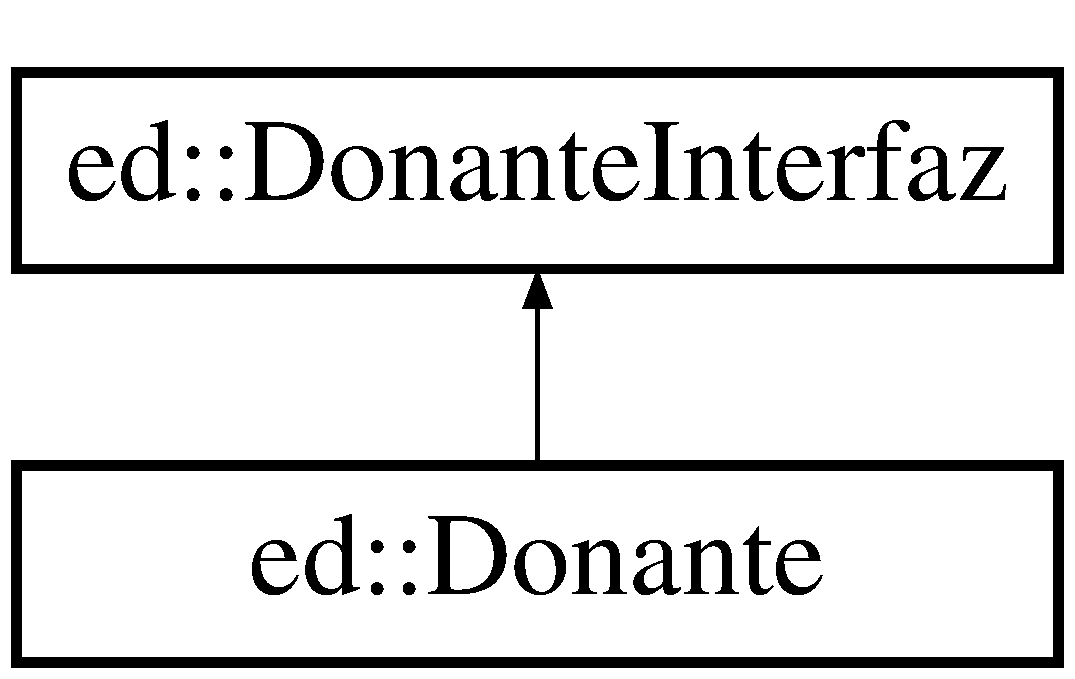
\includegraphics[height=2.000000cm]{classed_1_1DonanteInterfaz}
\end{center}
\end{figure}
\subsection*{Public Member Functions}
\begin{Indent}{\bf Métodos públicos de la clase Donante\-Interfaz}\par
\begin{DoxyCompactItemize}
\item 
virtual void \hyperlink{classed_1_1DonanteInterfaz_a4125f376530591b4f0a8f7d2f294ecb6}{set\-Nombre} (const string \&nombre)=0
\begin{DoxyCompactList}\small\item\em Asigna un valor \char`\"{}nombre\char`\"{} al nombre de un donante. \end{DoxyCompactList}\item 
virtual void \hyperlink{classed_1_1DonanteInterfaz_a6556974eb878ea122f6d2f6addf9fbfd}{set\-Apellido} (const string \&apellido)=0
\begin{DoxyCompactList}\small\item\em Asigna un valor \char`\"{}apellido\char`\"{} al apellido de un donante. \end{DoxyCompactList}\item 
virtual void \hyperlink{classed_1_1DonanteInterfaz_a313d06006b89e8754bd18e6ee6e712c9}{set\-Grupo\-Sanguineo} (const string \&grupo\-Sanguineo)=0
\begin{DoxyCompactList}\small\item\em Asigna un valor \char`\"{}grupo\-Sanguineo\char`\"{} al grupo\-Sanguineo de un donante. \end{DoxyCompactList}\item 
virtual void \hyperlink{classed_1_1DonanteInterfaz_ab75c31670ebf83b9cb081a026d2b943c}{set\-Factor\-R\-H} (const string \&factor\-R\-H)=0
\begin{DoxyCompactList}\small\item\em Asigna un valor \char`\"{}factor\-R\-H\char`\"{} al factor\-R\-H de un donante. \end{DoxyCompactList}\item 
virtual string \hyperlink{classed_1_1DonanteInterfaz_a907becd8ffab6ea63c026bec0666fa03}{get\-Nombre} () const =0
\begin{DoxyCompactList}\small\item\em Devuelve el nombre de un donante. \end{DoxyCompactList}\item 
virtual string \hyperlink{classed_1_1DonanteInterfaz_af318d1ba60b3ef9450218a30e980d3a6}{get\-Apellido} () const =0
\begin{DoxyCompactList}\small\item\em Devuelve el apellido de un donante. \end{DoxyCompactList}\item 
virtual string \hyperlink{classed_1_1DonanteInterfaz_a06fe986962a85b487c8e1c5525beec15}{get\-Grupo\-Sanguineo} () const =0
\begin{DoxyCompactList}\small\item\em Devuelve el grupo sanguineo de un donante. \end{DoxyCompactList}\item 
virtual string \hyperlink{classed_1_1DonanteInterfaz_ad6137e761b69b8fd085088a7a01cf5e2}{get\-Factor\-R\-H} () const =0
\begin{DoxyCompactList}\small\item\em Devuelve el factor R\-H de un donante. \end{DoxyCompactList}\end{DoxyCompactItemize}
\end{Indent}


\subsection{Detailed Description}
Definición de la clase \hyperlink{classed_1_1DonanteInterfaz}{Donante\-Interfaz}. 

\subsection{Member Function Documentation}
\hypertarget{classed_1_1DonanteInterfaz_af318d1ba60b3ef9450218a30e980d3a6}{\index{ed\-::\-Donante\-Interfaz@{ed\-::\-Donante\-Interfaz}!get\-Apellido@{get\-Apellido}}
\index{get\-Apellido@{get\-Apellido}!ed::DonanteInterfaz@{ed\-::\-Donante\-Interfaz}}
\subsubsection[{get\-Apellido}]{\setlength{\rightskip}{0pt plus 5cm}virtual string ed\-::\-Donante\-Interfaz\-::get\-Apellido (
\begin{DoxyParamCaption}
{}
\end{DoxyParamCaption}
) const\hspace{0.3cm}{\ttfamily [pure virtual]}}}\label{classed_1_1DonanteInterfaz_af318d1ba60b3ef9450218a30e980d3a6}


Devuelve el apellido de un donante. 

\begin{DoxyReturn}{Returns}
Apellido de un donate 
\end{DoxyReturn}
\begin{DoxyPrecond}{Precondition}
El donante debe existir anteriormente 
\end{DoxyPrecond}
\begin{DoxyPostcond}{Postcondition}
Ninguna 
\end{DoxyPostcond}


Implemented in \hyperlink{classed_1_1Donante_a3c47b3238b610ea3541161bc1a90d9f8}{ed\-::\-Donante}.

\hypertarget{classed_1_1DonanteInterfaz_ad6137e761b69b8fd085088a7a01cf5e2}{\index{ed\-::\-Donante\-Interfaz@{ed\-::\-Donante\-Interfaz}!get\-Factor\-R\-H@{get\-Factor\-R\-H}}
\index{get\-Factor\-R\-H@{get\-Factor\-R\-H}!ed::DonanteInterfaz@{ed\-::\-Donante\-Interfaz}}
\subsubsection[{get\-Factor\-R\-H}]{\setlength{\rightskip}{0pt plus 5cm}virtual string ed\-::\-Donante\-Interfaz\-::get\-Factor\-R\-H (
\begin{DoxyParamCaption}
{}
\end{DoxyParamCaption}
) const\hspace{0.3cm}{\ttfamily [pure virtual]}}}\label{classed_1_1DonanteInterfaz_ad6137e761b69b8fd085088a7a01cf5e2}


Devuelve el factor R\-H de un donante. 

\begin{DoxyReturn}{Returns}
factor\-R\-H de un donante 
\end{DoxyReturn}
\begin{DoxyPrecond}{Precondition}
El donante debe existir anteriormente 
\end{DoxyPrecond}
\begin{DoxyPostcond}{Postcondition}
Ninguna 
\end{DoxyPostcond}


Implemented in \hyperlink{classed_1_1Donante_a61c107f22340497f4bf5169997be5ddc}{ed\-::\-Donante}.

\hypertarget{classed_1_1DonanteInterfaz_a06fe986962a85b487c8e1c5525beec15}{\index{ed\-::\-Donante\-Interfaz@{ed\-::\-Donante\-Interfaz}!get\-Grupo\-Sanguineo@{get\-Grupo\-Sanguineo}}
\index{get\-Grupo\-Sanguineo@{get\-Grupo\-Sanguineo}!ed::DonanteInterfaz@{ed\-::\-Donante\-Interfaz}}
\subsubsection[{get\-Grupo\-Sanguineo}]{\setlength{\rightskip}{0pt plus 5cm}virtual string ed\-::\-Donante\-Interfaz\-::get\-Grupo\-Sanguineo (
\begin{DoxyParamCaption}
{}
\end{DoxyParamCaption}
) const\hspace{0.3cm}{\ttfamily [pure virtual]}}}\label{classed_1_1DonanteInterfaz_a06fe986962a85b487c8e1c5525beec15}


Devuelve el grupo sanguineo de un donante. 

\begin{DoxyReturn}{Returns}
grupo\-Sanguineo de un polinomio 
\end{DoxyReturn}
\begin{DoxyPrecond}{Precondition}
El donante debe existir anteriormente 
\end{DoxyPrecond}
\begin{DoxyPostcond}{Postcondition}
Ninguna 
\end{DoxyPostcond}


Implemented in \hyperlink{classed_1_1Donante_a6a6d49990afd2da9908df86462457049}{ed\-::\-Donante}.

\hypertarget{classed_1_1DonanteInterfaz_a907becd8ffab6ea63c026bec0666fa03}{\index{ed\-::\-Donante\-Interfaz@{ed\-::\-Donante\-Interfaz}!get\-Nombre@{get\-Nombre}}
\index{get\-Nombre@{get\-Nombre}!ed::DonanteInterfaz@{ed\-::\-Donante\-Interfaz}}
\subsubsection[{get\-Nombre}]{\setlength{\rightskip}{0pt plus 5cm}virtual string ed\-::\-Donante\-Interfaz\-::get\-Nombre (
\begin{DoxyParamCaption}
{}
\end{DoxyParamCaption}
) const\hspace{0.3cm}{\ttfamily [pure virtual]}}}\label{classed_1_1DonanteInterfaz_a907becd8ffab6ea63c026bec0666fa03}


Devuelve el nombre de un donante. 

\begin{DoxyReturn}{Returns}
Nombre de un donante 
\end{DoxyReturn}
\begin{DoxyPrecond}{Precondition}
El donante debe existir anteriormente 
\end{DoxyPrecond}
\begin{DoxyPostcond}{Postcondition}
Ninguna 
\end{DoxyPostcond}


Implemented in \hyperlink{classed_1_1Donante_a6ee5ef3051ee5e87aecefbbb68907d4a}{ed\-::\-Donante}.

\hypertarget{classed_1_1DonanteInterfaz_a6556974eb878ea122f6d2f6addf9fbfd}{\index{ed\-::\-Donante\-Interfaz@{ed\-::\-Donante\-Interfaz}!set\-Apellido@{set\-Apellido}}
\index{set\-Apellido@{set\-Apellido}!ed::DonanteInterfaz@{ed\-::\-Donante\-Interfaz}}
\subsubsection[{set\-Apellido}]{\setlength{\rightskip}{0pt plus 5cm}virtual void ed\-::\-Donante\-Interfaz\-::set\-Apellido (
\begin{DoxyParamCaption}
\item[{const string \&}]{apellido}
\end{DoxyParamCaption}
)\hspace{0.3cm}{\ttfamily [pure virtual]}}}\label{classed_1_1DonanteInterfaz_a6556974eb878ea122f6d2f6addf9fbfd}


Asigna un valor \char`\"{}apellido\char`\"{} al apellido de un donante. 


\begin{DoxyParams}{Parameters}
{\em apellido} & string pasado por referencia constante \\
\hline
\end{DoxyParams}
\begin{DoxyPrecond}{Precondition}
El donate debe existir anteriormente 
\end{DoxyPrecond}
\begin{DoxyPostcond}{Postcondition}
Ninguna 
\end{DoxyPostcond}


Implemented in \hyperlink{classed_1_1Donante_ae1404d01bdc865c03bfc179b408df4d7}{ed\-::\-Donante}.

\hypertarget{classed_1_1DonanteInterfaz_ab75c31670ebf83b9cb081a026d2b943c}{\index{ed\-::\-Donante\-Interfaz@{ed\-::\-Donante\-Interfaz}!set\-Factor\-R\-H@{set\-Factor\-R\-H}}
\index{set\-Factor\-R\-H@{set\-Factor\-R\-H}!ed::DonanteInterfaz@{ed\-::\-Donante\-Interfaz}}
\subsubsection[{set\-Factor\-R\-H}]{\setlength{\rightskip}{0pt plus 5cm}virtual void ed\-::\-Donante\-Interfaz\-::set\-Factor\-R\-H (
\begin{DoxyParamCaption}
\item[{const string \&}]{factor\-R\-H}
\end{DoxyParamCaption}
)\hspace{0.3cm}{\ttfamily [pure virtual]}}}\label{classed_1_1DonanteInterfaz_ab75c31670ebf83b9cb081a026d2b943c}


Asigna un valor \char`\"{}factor\-R\-H\char`\"{} al factor\-R\-H de un donante. 


\begin{DoxyParams}{Parameters}
{\em factor\-R\-H} & string pasado por referencia constante \\
\hline
\end{DoxyParams}
\begin{DoxyPrecond}{Precondition}
El donate debe existir anteriormente 
\end{DoxyPrecond}
\begin{DoxyPostcond}{Postcondition}
Ninguna 
\end{DoxyPostcond}


Implemented in \hyperlink{classed_1_1Donante_a724f1dcdf7a3cf78fd80151b30038c74}{ed\-::\-Donante}.

\hypertarget{classed_1_1DonanteInterfaz_a313d06006b89e8754bd18e6ee6e712c9}{\index{ed\-::\-Donante\-Interfaz@{ed\-::\-Donante\-Interfaz}!set\-Grupo\-Sanguineo@{set\-Grupo\-Sanguineo}}
\index{set\-Grupo\-Sanguineo@{set\-Grupo\-Sanguineo}!ed::DonanteInterfaz@{ed\-::\-Donante\-Interfaz}}
\subsubsection[{set\-Grupo\-Sanguineo}]{\setlength{\rightskip}{0pt plus 5cm}virtual void ed\-::\-Donante\-Interfaz\-::set\-Grupo\-Sanguineo (
\begin{DoxyParamCaption}
\item[{const string \&}]{grupo\-Sanguineo}
\end{DoxyParamCaption}
)\hspace{0.3cm}{\ttfamily [pure virtual]}}}\label{classed_1_1DonanteInterfaz_a313d06006b89e8754bd18e6ee6e712c9}


Asigna un valor \char`\"{}grupo\-Sanguineo\char`\"{} al grupo\-Sanguineo de un donante. 


\begin{DoxyParams}{Parameters}
{\em grupo\-Sanguineo} & string pasado por referencia constante \\
\hline
\end{DoxyParams}
\begin{DoxyPrecond}{Precondition}
El donate debe existir anteriormente 
\end{DoxyPrecond}
\begin{DoxyPostcond}{Postcondition}
Ninguna 
\end{DoxyPostcond}


Implemented in \hyperlink{classed_1_1Donante_a24dcea06d8dd84d596e115b8c94e8eb2}{ed\-::\-Donante}.

\hypertarget{classed_1_1DonanteInterfaz_a4125f376530591b4f0a8f7d2f294ecb6}{\index{ed\-::\-Donante\-Interfaz@{ed\-::\-Donante\-Interfaz}!set\-Nombre@{set\-Nombre}}
\index{set\-Nombre@{set\-Nombre}!ed::DonanteInterfaz@{ed\-::\-Donante\-Interfaz}}
\subsubsection[{set\-Nombre}]{\setlength{\rightskip}{0pt plus 5cm}virtual void ed\-::\-Donante\-Interfaz\-::set\-Nombre (
\begin{DoxyParamCaption}
\item[{const string \&}]{nombre}
\end{DoxyParamCaption}
)\hspace{0.3cm}{\ttfamily [pure virtual]}}}\label{classed_1_1DonanteInterfaz_a4125f376530591b4f0a8f7d2f294ecb6}


Asigna un valor \char`\"{}nombre\char`\"{} al nombre de un donante. 


\begin{DoxyParams}{Parameters}
{\em nombre} & string pasado por referencia constante \\
\hline
\end{DoxyParams}
\begin{DoxyPrecond}{Precondition}
El donate debe existir anteriormente 
\end{DoxyPrecond}
\begin{DoxyPostcond}{Postcondition}
Ninguna 
\end{DoxyPostcond}


Implemented in \hyperlink{classed_1_1Donante_a346b31e40b478d25c3e311de2ff2fb2c}{ed\-::\-Donante}.



The documentation for this class was generated from the following file\-:\begin{DoxyCompactItemize}
\item 
donante\-Interfaz.\-hpp\end{DoxyCompactItemize}

\chapter{File Documentation}
\hypertarget{funciones_8cpp}{\section{funciones.\-cpp File Reference}
\label{funciones_8cpp}\index{funciones.\-cpp@{funciones.\-cpp}}
}


Código de las funciones utilizadas en el menú  


{\ttfamily \#include $<$stdio.\-h$>$}\\*
{\ttfamily \#include $<$math.\-h$>$}\\*
{\ttfamily \#include $<$malloc.\-h$>$}\\*
{\ttfamily \#include \char`\"{}macros.\-hpp\char`\"{}}\\*
\subsection*{Functions}
\begin{DoxyCompactItemize}
\item 
\hypertarget{funciones_8cpp_a044c4eb65b70ed0ba39c3430280dce94}{void \hyperlink{funciones_8cpp_a044c4eb65b70ed0ba39c3430280dce94}{erastotenes} ()}\label{funciones_8cpp_a044c4eb65b70ed0ba39c3430280dce94}

\begin{DoxyCompactList}\small\item\em Función que aplica la Criba de Erastótenes para generar los números primos menores que un número dado. \end{DoxyCompactList}\item 
\hypertarget{funciones_8cpp_a0f757aeff74c4ba2fa53b0a07f9f1341}{void \hyperlink{funciones_8cpp_a0f757aeff74c4ba2fa53b0a07f9f1341}{factorial} ()}\label{funciones_8cpp_a0f757aeff74c4ba2fa53b0a07f9f1341}

\begin{DoxyCompactList}\small\item\em Función que calcula el factorial de un número natural. \end{DoxyCompactList}\end{DoxyCompactItemize}


\subsection{Detailed Description}
Código de las funciones utilizadas en el menú 
\hypertarget{funciones_8hpp}{\section{funciones.\-hpp File Reference}
\label{funciones_8hpp}\index{funciones.\-hpp@{funciones.\-hpp}}
}


Prototipos de las funciones utilizadas en el menú  


\subsection*{Functions}
\begin{DoxyCompactItemize}
\item 
\hypertarget{funciones_8hpp_a044c4eb65b70ed0ba39c3430280dce94}{void \hyperlink{funciones_8hpp_a044c4eb65b70ed0ba39c3430280dce94}{erastotenes} ()}\label{funciones_8hpp_a044c4eb65b70ed0ba39c3430280dce94}

\begin{DoxyCompactList}\small\item\em Función que aplica la Criba de Erastótenes para generar los números primos menores que un número dado. \end{DoxyCompactList}\item 
\hypertarget{funciones_8hpp_a0f757aeff74c4ba2fa53b0a07f9f1341}{void \hyperlink{funciones_8hpp_a0f757aeff74c4ba2fa53b0a07f9f1341}{factorial} ()}\label{funciones_8hpp_a0f757aeff74c4ba2fa53b0a07f9f1341}

\begin{DoxyCompactList}\small\item\em Función que calcula el factorial de un número natural. \end{DoxyCompactList}\end{DoxyCompactItemize}


\subsection{Detailed Description}
Prototipos de las funciones utilizadas en el menú 
\hypertarget{macros_8hpp}{\section{macros.\-hpp File Reference}
\label{macros_8hpp}\index{macros.\-hpp@{macros.\-hpp}}
}


Macros para el diseño de pantallas.  


\subsection*{Macros}
\begin{DoxyCompactItemize}
\item 
\hypertarget{macros_8hpp_a1e26748f72802cc32341cc3846db931f}{\#define {\bfseries L\-U\-G\-A\-R}(x, y)~printf(\char`\"{}\textbackslash{}033\mbox{[}\%d;\%d\-H\char`\"{},x,y)}\label{macros_8hpp_a1e26748f72802cc32341cc3846db931f}

\item 
\hypertarget{macros_8hpp_a79bf316fce01e63d76dddcdcbe72ab1c}{\#define {\bfseries B\-O\-R\-R\-A\-R}~printf(\char`\"{}\textbackslash{}33\mbox{[}2\-J\char`\"{})}\label{macros_8hpp_a79bf316fce01e63d76dddcdcbe72ab1c}

\item 
\hypertarget{macros_8hpp_ab86c2fc65d2b4c5205910f548828dcb9}{\#define {\bfseries P\-A\-R\-P\-A\-D\-E\-O}~printf(\char`\"{}\%c\mbox{[}5m\char`\"{},27)}\label{macros_8hpp_ab86c2fc65d2b4c5205910f548828dcb9}

\item 
\hypertarget{macros_8hpp_af2815fb445b50124864e3f2f958fac24}{\#define {\bfseries A\-P\-A\-G\-A}~printf(\char`\"{}\%c\mbox{[}0m\char`\"{},27)}\label{macros_8hpp_af2815fb445b50124864e3f2f958fac24}

\item 
\hypertarget{macros_8hpp_ac6cb5eae7b643f5d13c9d546e81dbcaf}{\#define {\bfseries I\-N\-V\-E\-R\-S\-O}~printf(\char`\"{}\%c\mbox{[}7m\char`\"{},27)}\label{macros_8hpp_ac6cb5eae7b643f5d13c9d546e81dbcaf}

\item 
\hypertarget{macros_8hpp_a3ab8b4157fd29a2336c702b26a967bb9}{\#define {\bfseries S\-U\-B\-R\-A\-Y\-A\-D\-O}~printf(\char`\"{}\%c\mbox{[}4m\char`\"{},27)}\label{macros_8hpp_a3ab8b4157fd29a2336c702b26a967bb9}

\item 
\hypertarget{macros_8hpp_af7eea73aeb56d77e1d56471ab214f8e2}{\#define {\bfseries I\-N\-T\-E\-N\-S\-I\-D\-A\-D}~printf(\char`\"{}\%c\mbox{[}1m\char`\"{},27)}\label{macros_8hpp_af7eea73aeb56d77e1d56471ab214f8e2}

\end{DoxyCompactItemize}


\subsection{Detailed Description}
Macros para el diseño de pantallas. 
%--- End generated contents ---

% Index
\newpage
\phantomsection
\addcontentsline{toc}{chapter}{Index}
\printindex

\end{document}
